% Compile this file with pdfLaTeX. Keep icml2026.sty in the same directory.
% ICML style source: https://icml.cc/Conferences/2026/AuthorInstructions
\documentclass{article}

\usepackage[T1]{fontenc}
\usepackage{microtype}
\usepackage{booktabs}
\usepackage{float}
\usepackage[hidelinks]{hyperref}
\newcommand{\theHalgorithm}{\arabic{algorithm}}
\usepackage[accepted]{icml2026}
\usepackage{pgfplots}
\pgfplotsset{compat=1.18}

\newcommand{\reporttitle}{In Context Learning with Qwen3}
\icmltitlerunning{\reporttitle}

% Use the course footer in place of the conference publication notice.
\makeatletter
\newcommand{\coursefootnote}{%
  \global\icml@noticeprintedtrue
  \begingroup
  \renewcommand{\thefootnote}{}%
  \begin{NoHyper}%
  \footnotetext{\emph{CS725 Project Report. November 25, 2026.}}%
  \end{NoHyper}%
  \endgroup
}
\makeatother

\begin{document}

\twocolumn[
  \icmltitle{\reporttitle}
  \begin{icmlauthorlist}
    \icmlauthor{Tejaroop Vasam (26M0812)}{}
    \icmlauthor{Abhiroop Kambhampati (26M0773)}{}\\
    \icmlauthor{Ashwanth Thimmareddy (26M0763)}{}
    \icmlauthor{Gangavamsam Poojith (26M0836)}{}
  \end{icmlauthorlist}
  \icmlkeywords{in-context learning, retrieval, Qwen3, text-to-SQL, long-context evaluation}
  \vskip 0.3in
]
\coursefootnote

\begin{abstract}

We study retrieval, output format, and prompt length in three Qwen3 models. We evaluate
classification, text-to-SQL on Spider and BIRD, and long-answer QA on CLAPNQ. On both SQL
benchmarks, BGE-M3 improved execution accuracy over random table selection for all three models.
On BIRD, Qwen3-8B answered five of nine questions correctly when retrieval included every reference
table. In the CLAPNQ stress test, mean ROUGE-L for Qwen3-8B declined from 51.6\% at 2K to 42.5\%
at 16K tokens.

\end{abstract}

\section{Introduction}

In-context learning (ICL) lets a model use demonstrations without updating its weights. Accuracy
can depend on the demonstrations, instructions, parser, and context supplied to the model. We
compare these factors on the same held-out items.

Our evaluation asks three questions. How much does output formatting explain the apparent IMDb
zero-shot deficit? Does retrieved evidence improve results compared with random or reference-derived
evidence? How does answer quality change when the same evidence appears at different positions in a
longer prompt?

\section{Related Work}

\citet{brown2020} demonstrated few-shot prompting with GPT-3 without weight updates.
\citet{min2022} found that randomizing demonstration labels often had little effect on
classification and multiple-choice tasks. The role of label space, input distribution,
and format motivates our IMDb prompt controls.

J.~\citet{liu2022} found that similarity-based demonstration selection could outperform
random sampling. We test this comparison with BGE-M3. Our CLAPNQ evidence-placement
experiment builds on N.~F.~\citet{liu2024}.

\newpage

\section{Methodology}

\subsection{Models, Data, and Token Accounting}

The available exports cover Qwen3-1.7B, 4B, and 8B \citep{yang2025}. All use NF4 weights and greedy
generation. Chat conditions disable thinking. The exports share seed 42, dataset settings, and
the BGE-M3 revision.

The classification pilot uses label-balanced samples from IMDb (40), Yelp Polarity (12), TREC (12),
and Yahoo Answers (20). We evaluate 12 development questions each for Spider \citep{yu2018} and
BIRD \citep{li2023}. CLAPNQ uses 12 answerable items with at least one reference of 50 words or
more \citep{rosenthal2025}.

Classification accepts a single distinct candidate label anywhere in the response, ignoring case.
Responses with absent or conflicting labels count as errors. Label coverage is the share of
responses yielding a prediction, including incorrect predictions.

The runner counts the rendered input IDs with the Qwen tokenizer and reserves completion tokens
within the native 32,768-token budget. It separately records retriever token counts. BGE-M3 uses
normalized dense embeddings with cosine similarity and supports 8,192 tokens per encoded text
\citep{chen2024}.

\subsection{Experimental Controls}

Classification compares zero-shot, random four-shot, nearest-neighbor retrieval at 2, 4, and 8
shots, and label-balanced retrieval from 200 training items. IMDb also varies ordering, format,
response budget, and review slice. Its oracle uses the held-out label to select demonstrations.

SQL controls vary the schema while holding the question fixed. Reference SQL identifies the oracle
tables and the budget for matched-count retrieval, while generated SQL is scored by execution on the
benchmark SQLite database.

For long answers, the retrieval pool contains the reference passage and 63 seeded distractors. The
stress protocol holds the question and relevant passage fixed, adds distractors to target four
prompt lengths, and moves the relevant passage to the front, middle, or end.

\clearpage

% Page 2

\section{Experiments}

\subsection{Classification and Demonstrations}

\begin{table}[H]
\centering
\caption{Pooled classification accuracy (\%) on the same 84 test items across IMDb, TREC, Yahoo
Answers, and Yelp Polarity. Each item contributes equally.}
\small
\begin{tabular*}{\columnwidth}{@{\extracolsep{\fill}}lrrr@{}}
\toprule
\textbf{Prompt} & \textbf{1.7B} & \textbf{4B} & \textbf{8B} \\
\midrule
Label-only zero-shot & 41.7 & 72.6 & 83.3 \\
Random four-shot & 59.5 & 81.0 & 88.1 \\
BGE-M3 four-shot & 82.1 & 85.7 & 88.1 \\
\bottomrule
\end{tabular*}
\end{table}

Qwen3-1.7B gained the most with BGE-M3 four-shot, rising from 35/84 with zero-shot prompting
to 69/84. IMDb and Yahoo improved at every model size. On IMDb, BGE-M3 four-shot achieved
36/40, 36/40, and 38/40 across the three models, compared with 27/40, 34/40, and 37/40
for random four-shot.

\paragraph{Qualitative analysis.}

Both four-shot conditions drew from the same training pool and used the same instruction.
Replacing random demonstrations with retrieved ones corrected 22 predictions for 1.7B and
introduced three new errors. For 8B, three gains and three losses yielded the same accuracy.

On TREC, adding demonstrations increased Qwen3-1.7B's label coverage from 10/12 to 12/12 and
its accuracy from 2/12 to 9/12. The model also adopted the demonstrations' format. Seven
outputs used a type prefix and five continued the question-and-label pattern. Incorrect
labels fell from eight to three, accounting for most of the accuracy gain.

\begin{table}[H]
\centering
\caption{Actual classification prompt lengths across the three exports. Entries are median (maximum)
tokens.}
\small
\begin{tabular*}{\columnwidth}{@{\extracolsep{\fill}}lrr@{}}
\toprule
\textbf{Dataset} & \textbf{Label-only 0} & \textbf{BGE-M3 8} \\
\midrule
IMDb & 298 (1,287) & 2,639.5 (5,660) \\
TREC & 59 (63) & 189.5 (208) \\
Yahoo & 170 (489) & 1,386.5 (1,900) \\
Yelp & 203 (821) & 1,713 (3,129) \\
\bottomrule
\end{tabular*}
\end{table}

The longest classification prompt used 17.3\% of the native budget. The 16-token generation
allowance kept the total below 5,700 tokens, even for that eight-shot prompt.

\newpage

\subsection{IMDb Zero-Shot Diagnosis}

\begin{table}[H]
\centering
\caption{IMDb classification accuracy (\%) on the same 40 reviews under four zero-shot conditions.}
\small
\begin{tabular*}{\columnwidth}{@{\extracolsep{\fill}}lrrr@{}}
\toprule
\textbf{Prompt} & \textbf{1.7B} & \textbf{4B} & \textbf{8B} \\
\midrule
Raw, 16 tokens & 10.0 & 30.0 & 62.5 \\
Raw, 64 tokens & 0.0 & 27.5 & 47.5 \\
Chat, same instruction & 75.0 & 85.0 & 90.0 \\
Label-only chat & 60.0 & 80.0 & 92.5 \\
\bottomrule
\end{tabular*}
\end{table}

The raw zero-shot prompt had a median of 280 tokens and a maximum of 1,269. All 40 raw 8B responses
reached the 16-token cap, and 13 contained neither sentiment label. With the same instruction in
chat format, label coverage rose from 27/40 to 39/40 and accuracy from 25/40 to 36/40. The label-only
instruction in chat gave 37/40 correct for 8B and lowered accuracy for the two smaller models
relative to the same-instruction chat arm. For 1.7B, the concise instruction yielded a label
on all 40 reviews and returned Negative on 36, including 16 of the 20 positive reviews.

The raw 64-token condition retained the same question and instruction. For 8B, 11 responses
contained neither label and another nine mentioned both. Accuracy fell to 19/40. The extra
generation budget gave raw responses more room to continue without reliably yielding a usable
sentiment judgment.

\paragraph{Qualitative analysis.}

Among 8B responses with an extractable label, 25/27 were correct in raw format and 36/39
were correct in chat format. The rates were similar once a label could be recovered. The
higher overall accuracy in chat came primarily from producing more usable labels. For 1.7B,
the shift toward Negative in label-only chat outweighed the gain in coverage.

The likelihood experiment compared the two candidate labels directly. Before calibration,
1.7B favored Negative on all 40 reviews and scored 20/40. We estimated its label preference
using content-free inputs, including an empty review, and subtracted that prior from the label
scores. This recovered 10 positive reviews at the cost of one negative review, yielding 29/40.
The same correction left 8B at 37/40.

\clearpage

% Page 3

\subsection{Retrieval and Executable SQL}

\begin{table}[H]
\centering
\caption{Execution accuracy (\%) on 12 matched prompts per SQL dataset.}
\small
\begin{tabular*}{\columnwidth}{@{\extracolsep{\fill}}lrrr@{}}
\toprule
\textbf{Schema condition} & \textbf{1.7B} & \textbf{4B} & \textbf{8B} \\
\midrule
Spider / random & 33.3 & 50.0 & 50.0 \\
Spider / BGE-M3 & 58.3 & 75.0 & 75.0 \\
Spider / oracle & 66.7 & 83.3 & 91.7 \\
Spider / full & 75.0 & 91.7 & 91.7 \\
Spider / full + 2 shots & 66.7 & 75.0 & 75.0 \\
BIRD / random & 16.7 & 25.0 & 25.0 \\
BIRD / BGE-M3 & 25.0 & 41.7 & 41.7 \\
BIRD / oracle & 25.0 & 50.0 & 58.3 \\
BIRD / full & 25.0 & 58.3 & 50.0 \\
\bottomrule
\end{tabular*}
\end{table}

BGE-M3 outperformed matched-count random tables at every model size on both benchmarks. Mean
reference-table recall was 83.3\% on each. On BIRD, retrieval found all reference tables for
nine of the 12 questions.

\paragraph{Qualitative analysis.}

Across the three models, 13 of the 27 BIRD trials with full table coverage were correct. Of
the 14 errors in those trials, 12 queries ran and returned the wrong results, and two failed
during execution. Nine of the 12 executed errors had the wrong row or column count. The other
three had the expected shape and different row values. All nine trials with incomplete table
coverage were incorrect. These patterns distinguish absent schema context from errors in query
construction after retrieval supplied the required tables.

On the 11 BIRD questions with a paired evidence ablation, 4B scored 6/11 with the evidence and 4/11
without it. The corresponding comparison was 5/11 versus 4/11 for 8B. Spider's full-schema two-shot
arm scored below full-schema zero-shot at all three sizes.

Schema retrieval also shortened the prompts. On Spider, the median fell from 250.5 tokens with
the full schema to 137 with matched-count BGE-M3. On BIRD it fell from 873 to 299.5 tokens.
Table 4 shows the corresponding changes in execution accuracy.

The evaluator runs the generated and reference queries on the full read-only SQLite database.
Spider compares returned rows with multiplicity and preserves their order when the reference
uses \texttt{ORDER BY}. BIRD compares sets of rows. This execution-based criterion accepts
different SQL expressions when their results agree under the benchmark's comparison rule.

\newpage

\subsection{Grounded Long-Answer QA}

\begin{table}[H]
\centering
\caption{Mean best-reference ROUGE-L F1 (\%) on 12 CLAPNQ questions. Scores are lexical overlap
measures.}
\small
\begin{tabular*}{\columnwidth}{@{\extracolsep{\fill}}lrrr@{}}
\toprule
\textbf{Passage condition} & \textbf{1.7B} & \textbf{4B} & \textbf{8B} \\
\midrule
No passage & 18.2 & 22.4 & 22.6 \\
Random passage & 13.5 & 18.5 & 15.6 \\
BGE-M3 passage & 40.8 & 45.7 & 43.2 \\
Gold passage & 40.8 & 45.7 & 43.2 \\
Gold + 2 shots & 33.4 & 48.7 & 50.0 \\
\bottomrule
\end{tabular*}
\end{table}

BGE-M3 ranked the annotated passage first for all 12 questions. The retrieved and gold prompts were
identical on every pair in the exports, which accounts for their equal scores. The candidate pool
includes the benchmark passage by design. The 12/12 result describes this shortlist and does not
measure open-corpus retrieval.

The gold passage raised ROUGE-L on each of the 12 questions relative to answering without a
passage, for all three models. Random selection drew the gold passage once, yielding identical
prompts on that item. On the other 11 questions the gold passage scored higher than the random
one for every model. With the gold passage fixed, adding two demonstrations increased mean overlap
for 4B and 8B and reduced it for 1.7B.

\paragraph{Qualitative analysis.}

All 33 responses to randomly selected distractor passages explicitly acknowledged that the
supplied evidence could not support an answer. Qwen3-1.7B and 8B withheld a substantive answer
in all 22 of their responses. Qwen3-4B provided an answer or partial answer from outside the
passage in two of its 11 responses, while acknowledging the evidence gap.

Without a passage, 8B attempted to answer all 12 questions directly. The change in response
behavior helps explain its lower ROUGE-L under random retrieval. ROUGE-L measures overlap
with an answer grounded in the annotated passage, so an appropriate abstention can score poorly
when the reference contains a substantive answer.

\clearpage

% Page 4

\subsection{Prompt Length and Evidence Position}

Four CLAPNQ questions were crossed with three evidence positions and four length targets.
For each question, longer prompts add passages from the same seeded distractor sequence. The
longest input used 29,900 tokens, with 384 tokens reserved for decoding within the
32,768-token context window.

\begin{table}[H]
\centering
\caption{Median actual input size and distractor count at each CLAPNQ length target.}
\small
\begin{tabular*}{\columnwidth}{@{\extracolsep{\fill}}lrr@{}}
\toprule
\textbf{Target} & \textbf{Input tokens} & \textbf{Distractors} \\
\midrule
2K & 1,904 & 6.0 \\
8K & 8,042.5 & 33.0 \\
16K & 16,253.5 & 66.5 \\
30K & 29,886 & 121.0 \\
\bottomrule
\end{tabular*}
\end{table}

\begin{figure}[H]
\centering
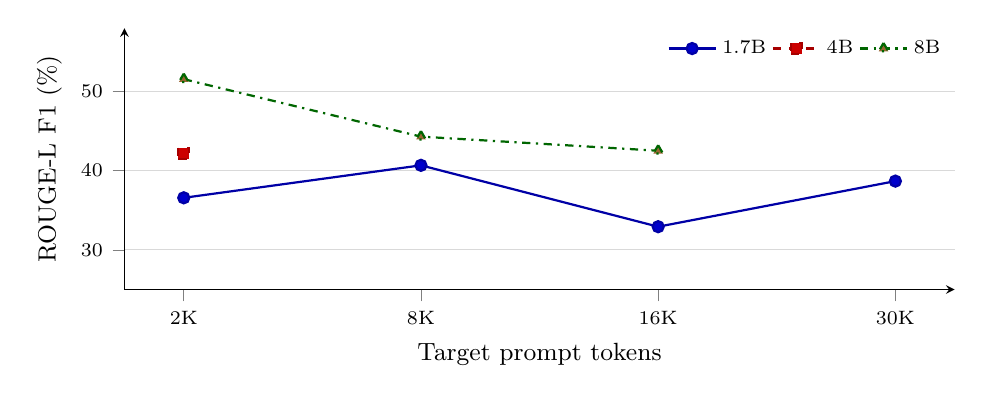
\begin{tikzpicture}
\begin{axis}[
    width=\columnwidth, height=4.9cm,
    xmin=-0.25, xmax=3.25, ymin=25, ymax=58,
    xtick={0,1,2,3}, xticklabels={2K,8K,16K,30K},
    ytick={30,40,50}, ymajorgrids, grid style={gray!30},
    axis lines=left, tick align=outside,
    xlabel={Target prompt tokens}, ylabel={ROUGE-L F1 (\%)},
    label style={font=\small}, tick label style={font=\scriptsize},
    legend style={font=\scriptsize, draw=none, fill=none, at={(1,1)}, anchor=north east},
    legend columns=3, every axis plot/.append style={thick, mark size=2pt},
]
\addplot+[blue!65!black,mark=*] coordinates {(0,36.5833) (1,40.6830) (2,32.9336) (3,38.6907)};
\addlegendentry{1.7B}
\addplot+[red!65!black,dashed,mark=square*] coordinates {(0,42.2189)};
\addlegendentry{4B}
\addplot+[green!40!black,dashdotted,mark=triangle*] coordinates {(0,51.5669) (1,44.3096)
(2,42.5277)};
\addlegendentry{8B}
\end{axis}
\end{tikzpicture}
\caption{Mean CLAPNQ ROUGE-L F1 across four questions and three evidence positions. Points
are shown for model and prompt length combinations with recorded scores.}
\label{fig:clapnq-stress}
\end{figure}

\paragraph{Qualitative analysis.}

For 8B, ROUGE-L declined in 10 of 12 matched comparisons from 2K to 16K. Averaging over the
three evidence positions, it fell on each of the four questions. The average response grew
from 93 to 112 words. The longer condition added distractors to the same evidence, so the
decline reflects the combined change in prompt length and surrounding text.

\newpage

\subsection{Evidence Placement and Answer Content}

\begin{table}[H]
\centering
\caption{Mean ROUGE-L F1 (\%) by evidence position on four CLAPNQ questions per row, for
model and length combinations with recorded scores.}
\small
\begin{tabular*}{\columnwidth}{@{\extracolsep{\fill}}lrrr@{}}
\toprule
\textbf{Model / target} & \textbf{Front} & \textbf{Middle} & \textbf{End} \\
\midrule
1.7B / 2K & 39.6 & 33.7 & 36.5 \\
1.7B / 8K & 42.8 & 43.7 & 35.5 \\
1.7B / 16K & 41.3 & 26.6 & 30.9 \\
1.7B / 30K & 45.3 & 28.7 & 42.1 \\
4B / 2K & 45.2 & 40.2 & 41.3 \\
8B / 2K & 48.0 & 52.4 & 54.3 \\
8B / 8K & 42.1 & 44.1 & 46.7 \\
8B / 16K & 46.1 & 39.2 & 42.3 \\
\bottomrule
\end{tabular*}
\end{table}

\paragraph{Qualitative analysis.}

At 16K, both 1.7B and 8B scored lowest with evidence in the middle. At 8K their lowest-scoring
positions differed. The results suggest that the benefit of a position depends on prompt
length and model.

At 16K, the annotated passage started near token 46 in the front condition, 7,731 in the
middle condition, and 16,048 in the end condition, using the median start index across the four
questions. The question followed the passage list in all three conditions. In both models,
the front position scored highest at 16K even though the relevant passage was farthest from
the question.

For Qwen3-8B from 2K to 16K, mean ROUGE-L precision fell from 45.9\% to 35.7\%, and mean
recall fell from 61.3\% to 55.6\%, using the best-matching reference for each response. The
longer responses shared a smaller proportion of their wording with the references and also
matched less of the reference wording. This pattern concerns lexical overlap. Judgments of
factual accuracy and evidence use require reading the responses against their sources.

\section{Conclusion}

BGE-M3 schema retrieval improved execution accuracy over matched-count random table selection on
Spider and BIRD. On BIRD, many incorrect queries ran successfully with complete table coverage,
which points to query construction as a separate source of error. On CLAPNQ, BGE-M3 recovered the
gold passage for all sampled questions, and the responses changed with the evidence supplied.

Classification prompts stayed well within the Qwen3 context window, and classification accuracy
varied with prompt format and demonstrations. In the CLAPNQ stress test, the effect of evidence
position varied across prompt lengths.

\clearpage

% Page 5

\section*{Team Contribution}

\textbf{Tejaroop Vasam (26M0812)} implemented classification sampling, zero-shot and few-shot
prompts, and the IMDb experiments on output format, generation budget, and label calibration.

\textbf{Abhiroop Kambhampati (26M0773)} implemented BGE-M3 embedding and similarity ranking for
classification demonstrations, SQL schemas and demonstrations, and CLAPNQ passages, as well as
top-\(k\) and label-balanced demonstration selection.

\textbf{Ashwanth Thimmareddy (26M0763)} implemented the gold, retrieved, and random passage conditions for CLAPNQ,
along with distractor construction, evidence placement, and prompt-token accounting for the
length sweep.

\textbf{Gangavamsam Poojith (26M0836)} integrated Spider and BIRD with their SQLite databases, implemented the
full-schema and oracle controls, and built read-only SQL execution scoring with
benchmark-specific result matching.

\section*{AI Usage}

We used AI to understand methods described in related research papers, clarify Python concepts and
library APIs, and research candidate benchmark datasets and their task formats.

\begin{thebibliography}{8}

\bibitem[Brown et al.(2020)]{brown2020}
Brown, T. B., Mann, B., Ryder, N., Subbiah, M., Kaplan, J. D., Dhariwal, P., Neelakantan, A.,
Shyam, P., Sastry, G., Askell, A., Agarwal, S., Herbert-Voss, A., Krueger, G., Henighan, T.,
Child, R., Ramesh, A., Ziegler, D. M., Wu, J., Winter, C., \ldots{} Amodei, D. (2020).
Language models are few-shot learners. In H. Larochelle, M. Ranzato, R. Hadsell, M. F. Balcan,
\& H. Lin (Eds.), \emph{Advances in Neural Information Processing Systems}
(Vol.~33, pp.~1877--1901). Curran Associates.
\href{https://proceedings.neurips.cc/paper_files/paper/2020/hash/1457c0d6bfcb4967418bfb8ac142f64a-Abstract.html}{NeurIPS proceedings}

\bibitem[Chen et al.(2024)]{chen2024}
Chen, J., Xiao, S., Zhang, P., Luo, K., Lian, D., \& Liu, Z. (2024). M3-Embedding: Multi-linguality,
multi-functionality, multi-granularity text embeddings through self-knowledge distillation.
\emph{Findings of ACL}, 2318--2335.
\url{https://aclanthology.org/2024.findings-acl.137/}

\bibitem[Li et al.(2023)]{li2023}
Li, J., Hui, B., Qu, G., Yang, J., Li, B., Li, B., Wang, B., Qin, B., Cao, R., Geng, R., Huo, N.,
Zhou, X., Ma, C., Li, G., Chang, K. C.-C., Huang, F., Cheng, R., \& Li, Y. (2023). Can LLM already
serve as a database interface? A big bench for large-scale database grounded text-to-SQLs.
\emph{Advances in Neural Information Processing Systems, 36}.
\url{https://arxiv.org/abs/2305.03111}

\bibitem[Liu et al.(2022)]{liu2022}
Liu, J., Shen, D., Zhang, Y., Dolan, B., Carin, L., \& Chen, W. (2022). What makes good in-context
examples for GPT-3? In E. Agirre, M. Apidianaki, \& I. Vuli\'{c} (Eds.),
\emph{Proceedings of Deep Learning Inside Out (DeeLIO 2022)} (pp.~100--114).
Association for Computational Linguistics. \url{https://doi.org/10.18653/v1/2022.deelio-1.10}

\bibitem[Liu et al.(2024)]{liu2024}
Liu, N. F., Lin, K., Hewitt, J., Paranjape, A., Bevilacqua, M., Petroni, F., \& Liang, P. (2024).
Lost in the middle: How language models use long contexts. \emph{Transactions of the Association
for Computational Linguistics, 12}, 157--173.
\url{https://doi.org/10.1162/tacl_a_00638}

\bibitem[Min et al.(2022)]{min2022}
Min, S., Lyu, X., Holtzman, A., Artetxe, M., Lewis, M., Hajishirzi, H., \& Zettlemoyer, L. (2022).
Rethinking the role of demonstrations: What makes in-context learning work?
In Y. Goldberg, Z. Kozareva, \& Y. Zhang (Eds.), \emph{Proceedings of the 2022 Conference on
Empirical Methods in Natural Language Processing} (pp.~11048--11064).
Association for Computational Linguistics. \url{https://doi.org/10.18653/v1/2022.emnlp-main.759}

\bibitem[Rosenthal et al.(2025)]{rosenthal2025}
Rosenthal, S., Sil, A., Florian, R., \& Roukos, S. (2025). CLAPnq: Cohesive long-form answers from
passages in Natural Questions for RAG systems. \emph{Transactions of the Association for
Computational Linguistics, 13}, 53--72.
\url{https://aclanthology.org/2025.tacl-1.3/}

\bibitem[Yang et al.(2025)]{yang2025}
Yang, A., Li, A., Yang, B., Zhang, B., Hui, B., Zheng, B., Yu, B., Gao, C., Huang, C., Lv, C.,
Zheng, C., Liu, D., Zhou, F., Huang, F., Hu, F., Ge, H., Wei, H., Lin, H., Tang, J., ... \& Qiu, Z.
(2025). Qwen3 technical report. \emph{arXiv}.
\url{https://arxiv.org/abs/2505.09388}

\bibitem[Yu et al.(2018)]{yu2018}
Yu, T., Zhang, R., Yang, K., Yasunaga, M., Wang, D., Li, Z., Ma, J., Li, I., Yao, Q., Roman, S.,
Zhang, Z., \& Radev, D. (2018). Spider: A large-scale human-labeled dataset for complex and
cross-domain semantic parsing and text-to-SQL task. \emph{Proceedings of EMNLP}, 3911--3921.
\url{https://arxiv.org/abs/1809.08887}

\end{thebibliography}

\end{document}
